\section{Controlling the Virtual Rover NEW}
\label{sec:control_vr_model}

\begin{figure}[!h]
	\centering
	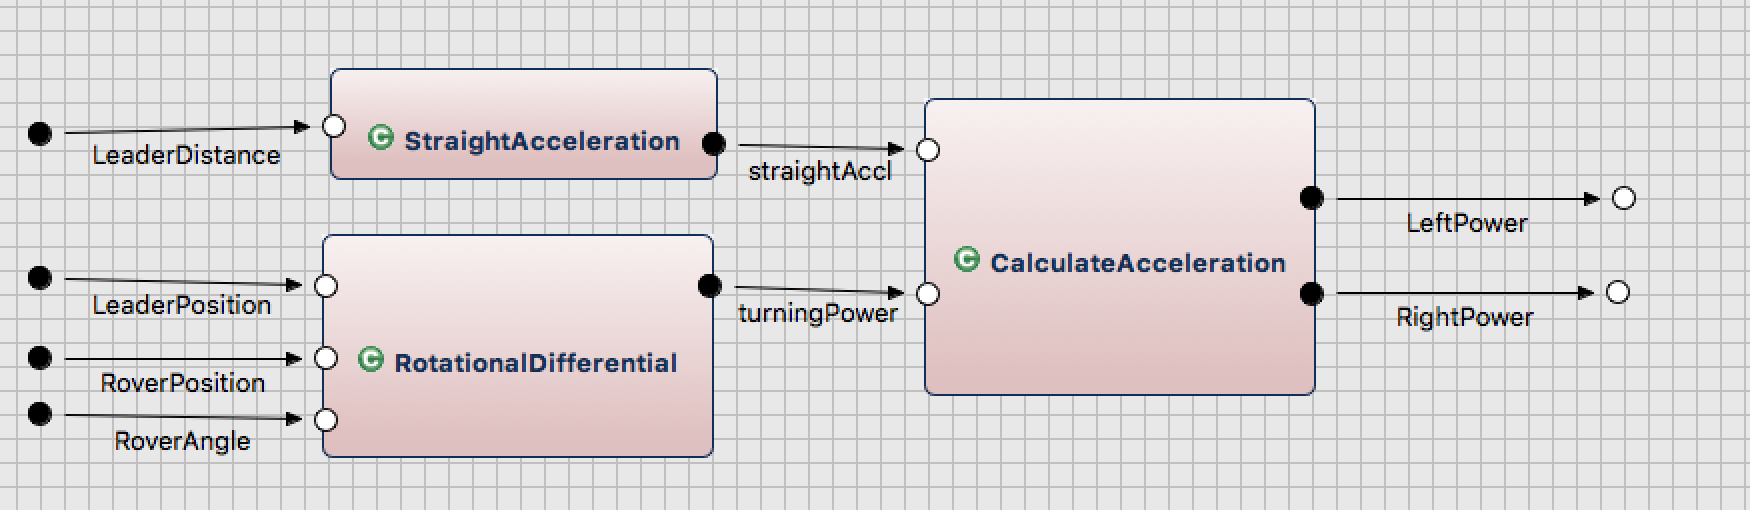
\includegraphics[width=1\textwidth]{images/acc.png}
	\caption{The controller for the Virtual Rover}
	\label{fig:acc}
\end{figure}

In \fig\ref{fig:acc} we depict the top-level model of the controller for the
follower vehicle. The controller is meant to operate in a loop by reading the
 {distance} to
the leader rover, the GPS coordinates of the leader (\textit{LeaderPosition})
and the rover's own (\textit{RoverPosition}) GPS coordinates as well as its own
orientation with respect to the north (\textit{RoverAngle}).
Note that the inputs to the model appear in \fig\ref{fig:acc}  as small black
circles, while the outputs have the same shape but are white. The power provided
to the wheels is constantly updated to reflect the changes in the input values
to the controller.

The controller for the virtual rover is composed by three \af components,
as explained in the next sections.

\subsection{Component StraightPower}
The \textsf{StraightPower} component is responsible for calculating the required
 forward power based on the distance to the leader.

This component is composed of two components as shown in \fig\ref{fig:straight}.
The component \textit{CalculateDistanceError} calculates the \textit{error} with
respect to the ideal distance with the leader. For the proposed challenge, the
follower was required to remain in the distance range between 12 and 15 from the
leader. We have thus taken the ideal distance as the average of these two
values, i.e. 13.5. This is a constant and can be easily changed to allow for different
ranges.

\begin{figure}[!h]
	\centering
	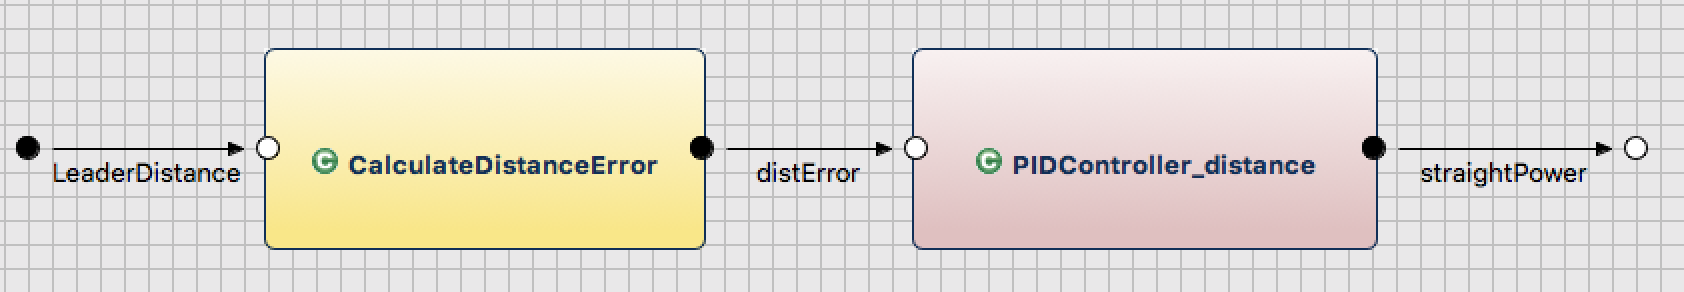
\includegraphics[width=1\textwidth]{images/straight.png}
	\caption{Component for calculating required forward power.}
	\label{fig:straight}
\end{figure}


We then use this \textit{error} and feed it to a PID controller for calculating
the power to be directed forward. The general equation for a PID controller
is\levi{explain in one sentence what this equation means}:
\begin{equation}
u = K_Pe + K_II + K_DD
\label{formula:pidController}
\end{equation}

For calculating the forward power we have used the following constant values: $K_P = 5$, $K_I=1.5$, $K_D=30$.

\subsection{Component RotationalDifferential}

The rover turns when the left and right wheels rotate at different speeds. The
magnitude of the difference is proportional to the turning angle.

When the leader turns the follower also has to turn in order to follow the
leader. In order to achieve this the \textsf{RotationalDifferential} component
calculates the required difference between the power applied to the right and
the left wheel to turn the rover to provide the correct turning angle.

The component \textsf{bearingAngle} calculates the bearing of the leader with
respect to north when seen from the follower. This calculation uses the GPS
positions of the follower and the leader. We then calculate the
\textit{angleError} i.e., the difference between the orientation of the follower
(with respect to north) and the bearing angle. This
\textit{angleError} is then passed onto another PID controller in order to
calculate the required difference in power sent to the rover's right and left
wheels. The sign of this value decides the direction of the turning.

\begin{figure}[!h]
	\centering
	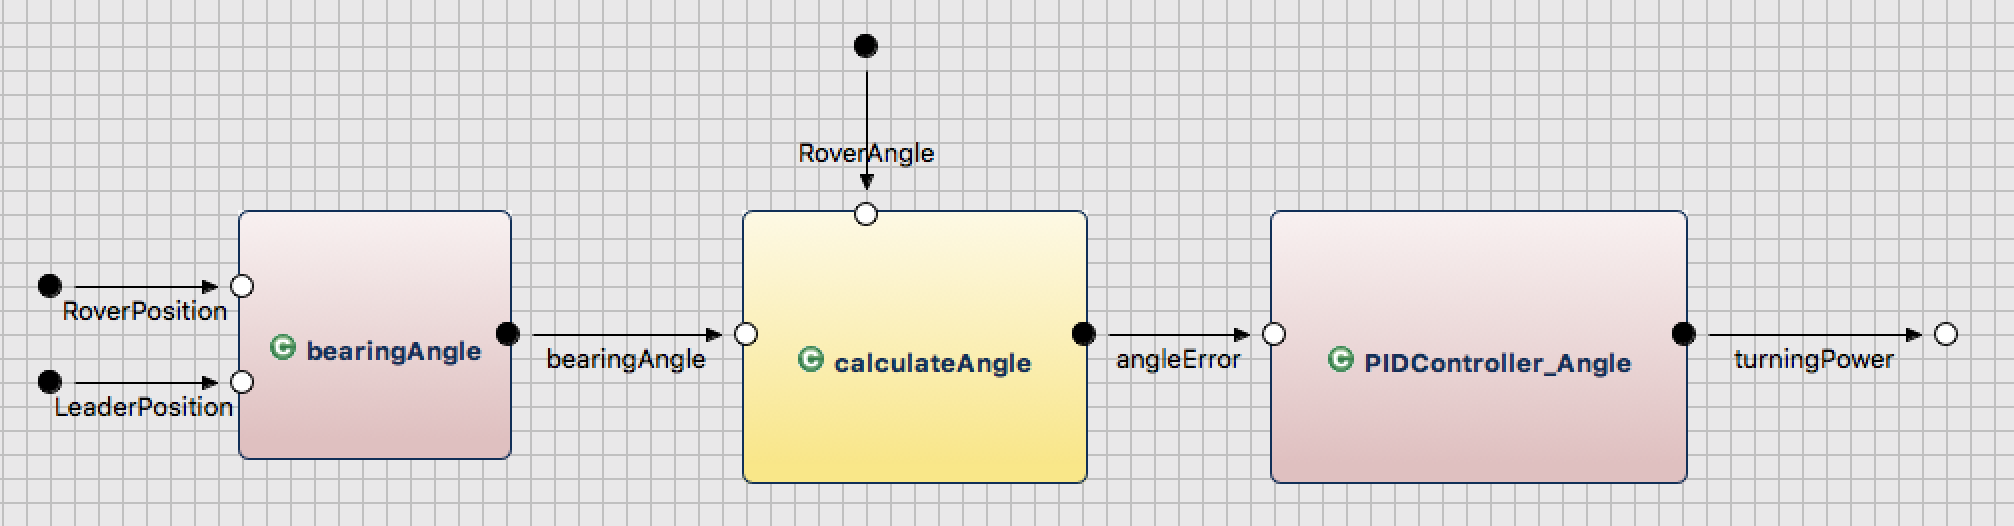
\includegraphics[width=1\textwidth]{images/rotation.png}
	\caption{Component for calculating the differential power.}
	\label{fig:rotation}
\end{figure}

The constants used of the PID controller (equation
\ref{formula:pidController}) for calculating the rotational differential are:
$K_P = 2$, $K_I=0.75$, $K_D=10$.

\subsection{Component CalculateFinalPower}
The \textsf{CalculateFinalPower} component takes the forward power and
\levi{rotational?} differential, and outputs the final power to apply to the
right and left wheels.
In addition to calculating the values for the right and left power, the
component also normalizes the amount of power provided in case the calculated
value exceeds the maximum.

The environment of the rover challenge proposed by the MDETools workshop
provides at the end of a run of the system \levi{can you write here how long
each run lasts?} the percentage of time during which the rover was within the
expected distance limits. The system we developed consistently
stays within these limits over 70\% of the runs we have attempted. Although we
have not tuned the values of the PID controller further, we believe even better results could be achieved.
The \af models we have used for the challenge can be downloaded
at~\cite{af3_mdetools}. For readers interested in further experimentation,
instructions accompanying the model provide the steps on how to install and
deploy the software.
